\section{背景介绍、系统工作原理和光路结构}

\subsection{凯尔纳目镜的历史背景}

目镜是望远镜、显微镜等光学仪器中直接与人眼接触的光学元件，其性能直接影响最终的观测体验。早期目镜设计以惠更斯目镜（Huygens Eyepiece）和冉斯登目镜（Ramsden Eyepiece）为代表，但这两种设计均存在明显的色差问题，成像质量有限。

1849年，德国光学家卡尔·凯尔纳（Carl Kellner）在冉斯登目镜的基础上提出了改良方案：将原来的单片目镜替换为消色差双合镜（Achromatic Doublet），由此诞生了凯尔纳目镜。这一改进使目镜的色差得到有效校正，视场角也扩大至40°～50°，成像质量相比早期设计有了质的飞跃\cite{Kingslake2010,Smith2008,Rutten2002}。时至今日，凯尔纳目镜因其结构简单、成本低廉、色差校正较好的特点，仍被广泛应用于入门级天文望远镜和双筒望远镜中，是初学者最常接触的目镜类型之一。

从光学系统设计角度看，目镜并不是单独成像的摄影镜头，而是与前方物镜共同组成完整的目视系统。物镜首先将远处目标成实像，目镜再将该实像放大并以近似平行光形式送入人眼。因此，目镜设计不仅要关注自身的焦距、视场和像差，还要兼顾出瞳位置、人眼瞳孔尺寸、观察舒适性以及与物镜焦平面的匹配关系。对于入门级或教学型望远镜而言，凯尔纳目镜在成像质量、加工难度和成本之间具有较好的折中，因此适合作为本次光学系统设计的研究对象。

与更复杂的广角目镜相比，凯尔纳目镜的镜片数较少，透过率较高，结构公差也相对容易控制；与简单的惠更斯或冉斯登目镜相比，它又通过消色差双合镜改善了轴向色差和部分轴外像差。这种“低复杂度但具备基本像差校正能力”的特点，使其非常适合用于学习光学系统建模、评价函数构造、像差平衡和公差分析的完整流程。

\subsection{凯尔纳目镜的光学结构与工作原理}

凯尔纳目镜由三片镜片组成，其光学结构如下：

\begin{itemize}
\item
  场镜（Field Lens）：位于焦平面附近，通常采用单片平凸透镜（平面朝向物方）。其主要作用是将边缘视场的光线折向光轴，使光线能够顺利通过后方的双合镜组，同时将出瞳位置调整至适合人眼观察的距离，扩大可用表观视场。
\item
  目镜组（Eye Lens，消色差双合镜）：由冕牌玻璃（Crown Glass，如BK7）和火石玻璃（Flint Glass，如F2）胶合而成。双合镜是目镜的核心光学元件，主要负责将来自场镜的发散光线准直为平行光束射向人眼，同时通过两种玻璃的色散互补对轴上色差进行校正。
\end{itemize}

从光路角度来看，使用时光线从望远镜物镜汇聚后在焦平面形成实像，该实像作为凯尔纳目镜的物面。光线先经过场镜进行视场整合，再进入消色差双合镜组，最终以平行光束出射并被人眼接收。整个光学系统等效于一个放大镜，人眼位于目镜的后焦点（出瞳）处观察虚像。

场镜与目镜组的分工是凯尔纳结构能够保持简洁的关键。场镜靠近物方焦平面，主要影响边缘视场光线高度和主光线走向，可用于改善视场利用率和出瞳位置；消色差双合镜靠近人眼一侧，承担主要会聚与色差校正任务。通过两种不同色散玻璃组合，双合镜可以使F光、d光和C光在轴上位置尽量接近，从而减小白光观察时的彩色边缘。与此同时，透镜曲率、空气间隔和光阑位置还会共同影响彗差、像散、场曲和畸变，需要在优化过程中进行综合平衡。

对于目视系统，出瞳是一个非常重要的设计量。若出瞳距离过短，观察者眼睛必须非常靠近目镜，舒适性较差；若出瞳位置过远或出瞳直径与人眼瞳孔不匹配，则可能导致视场截断或光能利用率下降。本设计采用4 mm入瞳直径，并在后续优化中关注出瞳直径、出瞳位置和相对照度，以保证系统不仅在像面评价指标上表现良好，也具有合理的观察体验。

与冉斯登目镜相比，凯尔纳目镜的主要优势在于：消色差双合镜对轴上色差（轴向色差）的校正能力显著更强；视场角更大（可达40°～50°）；出瞳距离（Eye Relief）更为舒适，一般可达10 mm以上。其主要不足在于：在较大视场角下仍存在一定的场曲、彗差和轴外色差；对于短焦距目镜，场镜离焦平面较近，镜面上的灰尘和划痕容易被人眼察觉；此外，内反射鬼像（Ghost Image）问题也较为突出。

\subsection{主要光学参数定义}

在进行凯尔纳目镜的设计与评估时，涉及以下主要光学参数\cite{Yu2016,Mu2000,Hecht2017}：

\begin{itemize}
\item
  焦距（Focal Length, EFL）：目镜的有效焦距，决定了目镜的放大率。望远镜的总放大倍数等于物镜焦距与目镜焦距之比。
\item
  表观视场角（Apparent Field of View, AFOV）：从出瞳处观察到的视场角范围，凯尔纳目镜一般为40°～50°，本设计取\(\pm 22.5^\circ\)（共45°）。
\item
  入瞳直径（Entrance Pupil Diameter）：进入目镜系统的有效光束直径。本设计取4 mm，用于控制光束口径、通光能力和后续像质评价的光线范围。
\item
  出瞳直径（Exit Pupil Diameter）：光束离开目镜时的直径，一般应与人眼瞳孔直径（白天约3 mm，夜间约5～7 mm）匹配，以充分利用光能。
\item
  出瞳距离（Eye Relief）：出瞳位置到目镜最后一片镜面顶点的距离，舒适的出瞳距离一般不低于10 mm，佩戴眼镜的观测者需要更大的出瞳距离（约15 mm以上）。
\item
  场曲（Field Curvature）：不同视场的最佳成像面不在同一平面上时产生的像差。场曲会使中心清晰时边缘离焦，或边缘清晰时中心离焦，是目镜设计中需要重点平衡的轴外像差。
\item
  像散（Astigmatism）：轴外物点在切向和弧矢方向形成两个不同焦点的现象。像散会使边缘视场点像拉长，影响星点或细节边缘的清晰度。
\item
  畸变（Distortion）：视场边缘图像相对于理想位置的偏移量，采用F-Tan(\(\theta\))畸变定义，一般要求不超过5\%。
\item
  相对照度（Relative Illumination）：边缘视场照度与轴上视场照度的比值。相对照度过低会造成边缘暗角，影响目视观察的均匀性。
\item
  点列图RMS半径（RMS Spot Radius）：用于衡量几何光线在像面上的弥散程度。RMS半径越小，说明光线聚焦越集中，几何像质越好。
\item
  调制传递函数（Modulation Transfer Function, MTF）：衡量光学系统在不同空间频率下的对比度传递能力，是评价成像质量的核心定量指标。
\item
  RMS波前误差（RMS Wavefront Error）：实际波前与理想球面波前的均方根偏差，按瑞利判据，当RMS波前误差小于\(\lambda\)/14（约0.07\(\lambda\)）时，系统接近衍射极限。
\end{itemize}

\subsection{本设计的目标与技术路线}

本设计的目标是在保持凯尔纳目镜三片式基本结构的前提下，获得有效焦距为30 mm、最大半视场角为\(\pm 22.5^\circ\)、入瞳直径为4 mm的目视光学系统。该指标既保留了凯尔纳目镜常见的中等视场特点，又避免因过分追求大视场而显著增加像差校正难度。设计过程中采用F光、d光和C光进行复色光分析，以d光作为主波长，并通过五个归一化视场对轴上至边缘视场进行均衡评价。

总体技术路线可概括为：首先依据经典凯尔纳目镜结构建立初始模型，确定透镜面序、材料组合、孔径和视场设置；其次在Zemax中构造评价函数，以有效焦距、系统长度、厚度边界和RMS点列半径为主要约束；然后通过局部优化、锤形优化和人工微调逐步改善像质；最后利用点列图、MTF、场曲畸变、相对照度、波前误差、图像模拟和公差分析对最终结果进行综合评价。通过这一流程，可以较完整地体现从初始结构选择到工程可制造性验证的光学设计思路。

\begin{figure}[H]
  \centering
  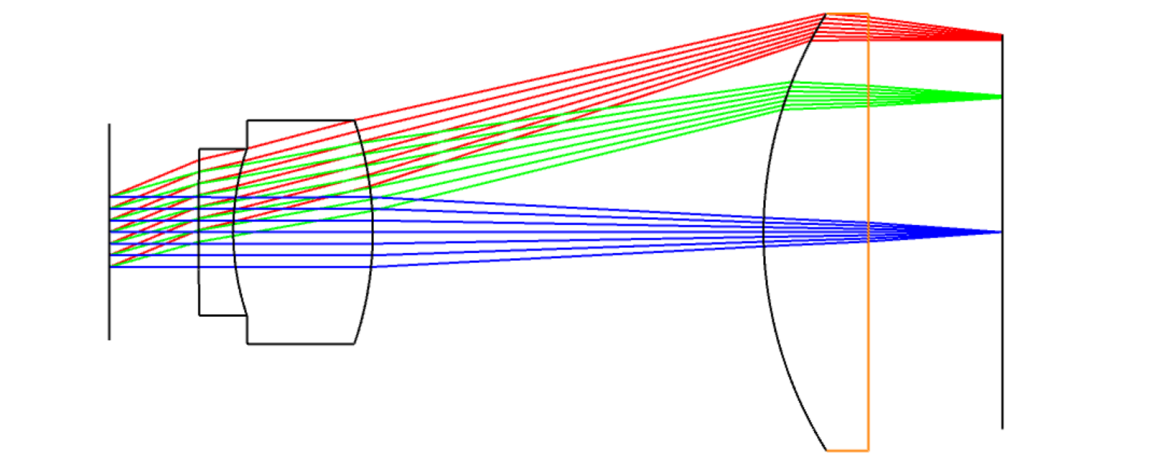
\includegraphics[width=0.95\textwidth]{chapters/chapter1/figures/2D_layout.png}
  \caption{凯尔纳目镜光路结构示意图（Zemax 2D布局图，初始结构）}
  \label{fig:chapter1-2d-layout}
\end{figure}
